\documentclass{article}

\usepackage{amsmath}
\usepackage{color}
\usepackage[hidelinks]{hyperref}
\usepackage{listings}
\usepackage{tikz}
\usepackage{tikz-qtree}
\usepackage{verbatim}

% Colors copied from https://stackoverflow.com/questions/3175105/
\definecolor{dkgreen}{rgb}{0,0.6,0}
\definecolor{gray}{rgb}{0.5,0.5,0.5}
\definecolor{mauve}{rgb}{0.58,0,0.82}

\lstset{
	aboveskip=5mm,
	belowskip=5mm,
	basicstyle={\large\ttfamily},
	columns=flexible,
	language=Lisp,
	numbers=left,
	showstringspaces=false,
	% Style copied from https://stackoverflow.com/questions/3175105/
	numberstyle=\normalsize\color{gray},
	keywordstyle=\color{blue},
	commentstyle=\color{dkgreen},
	stringstyle=\color{mauve},
}

\bibliographystyle{acm}

\title{The Ergonomics of Faceted Execution (full draft)}
\author{Ian Fisher}
\date{25 March 2019}

\begin{document}
\maketitle

\begin{abstract}
This thesis draft reviews faceted execution, a programming-language mechanism for enforcing privacy policies. I discuss several issues that could hinder the use of faceted execution in actual software development (efficiency, type safety, compatibility with non-faceted code), and review methods of mitigating these issues (abstract interpretation, static typing, Racket's \texttt{\#lang} mechanism). I present a prototype implementation of an extension to the existing \textsc{Racets} system \cite{racets} that integrates faceted execution into the Racket programming language.
\end{abstract}

\tableofcontents



\section{Introduction}
\subsection{Faceted execution\label{sec:facets}}
Software often deals with data which is governed by some privacy policy. On a social media website, for instance, a user's contact information may only be visible to the user's friends. For a bank or healthcare website, the enforcement of privacy policies may have serious legal and ethical consequences. However, implementing privacy policies in code can be tedious and error-prone, as the privacy logic tends to become coupled to the application logic. Faceted execution is a programming-language mechanism that aims to ease the implementation of privacy policies by decoupling an application's privacy policy from its logic.

Programs written with faceted execution operates on special data structures called facets, which enclose sensitive data. A facet is a tuple of the form $\langle l\ ?\ v_H : v_L \rangle$ where $l$ is a label, $v_H$ is the high-confidentiality value, and $v_L$ is the low-confidentiality value. $v_H$ can only be accessed by observers that match the facet's label; other observers can only see $v_L$, which is typically a default value like $0$ or \texttt{null}.

Faceted execution allows privacy policies to be expressed separately from the implementation of the program, meaning that changes to the privacy policy can be made reliably with minimal modification of the application logic. Faceted execution is thus an implementation of policy-agnostic programming \cite{faceted}.

Full support of faceted execution requires changes to core language mechanisms like function application. Concretely, if the function \texttt{square-root} were applied to the facet $\langle l \ ?\ 42 : 0 \rangle$, it must return the facet $\langle l \ ?\ \texttt{square-root}(42) : \texttt{square-root}(0) \rangle$, ensuring that the faceted value remains protected by the privacy policy, even if \texttt{square-root} is totally oblivious to the policy. Without changes to the mechanics of function application, a privacy-agnostic version of \texttt{square-root} would either choke on faceted input, inadvertently reveal sensitive data, or both.

Researchers have adopted different strategies to implement faceted execution. One strategy is to design a new programming language with faceted-execution primitives built-in. This is the strategy adopted by the Jeeves programming language \cite{jeeves}. Another strategy is to use syntactic macros to graft faceted execution on to an existing language, provided that the language's macro system is rich enough to support it. The \textsc{Racets} programming language adopts the latter strategy, by augmenting the Racket language with syntactic macros \cite{racets}.

The following subsections will present an overview of the mechanics of faceted execution specific to the \textsc{Racets} programming language, but the concepts are general enough to apply to other implementations of faceted execution.


\subsubsection{A simple example of faceted execution}
Policies, which govern access to sensitive data, are declared with the \texttt{let-label} form in \textsc{Racets}:

\begin{lstlisting}
(define alice-policy
  (let-label l (lambda (x) (equal? x "Alice")) l))

(define bob-policy
  (let-label l (lambda (x) (equal? x "Bob")) l))
\end{lstlisting}

The two declarations in the source code above create two policies and bind them to the names \texttt{alice-policy} and \texttt{bob-policy}. Note the somewhat idiomatic usage of the \texttt{let-label} form: the general syntax is \texttt{(let-label name value body)}, which binds \texttt{name} to \texttt{value} and evaluates \texttt{body} with this new binding. In the two declarations above, the body is simply the label name itself, so that the \texttt{let-label} form as a whole evaluates to the label.

The policies enforce that only entities identifying themselves as ``Alice'' or ``Bob'', respectively, may view the high-confidentiality value of any facet protected by the policies.

A faceted data value is created with the \texttt{fac} form:

\begin{lstlisting}
(define my-facet (fac alice-policy 42 0))
\end{lstlisting}

\texttt{my-facet} is defined with Alice's policy, the high-confidentiality value $42$, and the low-confidentiality value $0$.

The \texttt{obs} form is used to view the value of a facet:

\begin{lstlisting}
(obs alice-policy "Alice" my-facet)
\end{lstlisting}

The expression above will evaluate to $42$, as the argument \texttt{"Alice"} satisfies the facet's policy. By contrast, the expression below will evaluate to $0$ since \texttt{"Bob"} does not satisfy the facet's policy.

\begin{lstlisting}
(obs alice-policy "Bob" my-facet)
\end{lstlisting}

The policy passed to a facet must match the policy that the facet was created with. In the case that the facets do not match, \texttt{obs} functions as a no-op. Each of the two calls to \texttt{obs} below, for instance, will simply return \texttt{my-facet} unchanged.

\begin{lstlisting}
(obs bob-policy "Alice" my-facet)
(obs bob-policy "Bob" my-facet)
\end{lstlisting}

The forms \texttt{let-label}, \texttt{fac}, and \texttt{obs} comprise the primitive operations of faceted execution in \textsc{Racets}.


\subsubsection{An example of nested facets}
Faceted values may be nested for more fine-grained control over the views of the data that are available. While a single facet only encloses two different views of the data, a nested facet may enclose an arbitrary number of views. Alice could define a nested facet that specifies her location in three degrees of granularity:

\begin{lstlisting}
(define location-facet
  (fac alice-policy
    "370 Lancaster Ave, Haverford PA"
    (fac bob-policy
      "Haverford, PA"
      "Pennsylvania")))
\end{lstlisting}

Alice is able to view the full street address of her location. Bob (or anyone else satisfying Bob's policy) may see her town, and anyone else may only see her state of residence. The structure of the nested facet may be visualized as a tree, where the right branches are the high-confidentiality values, the left branches are the low-confidentiality values, the leaves are the non-faceted values, and the internal nodes are the policies:

\begin{center}
	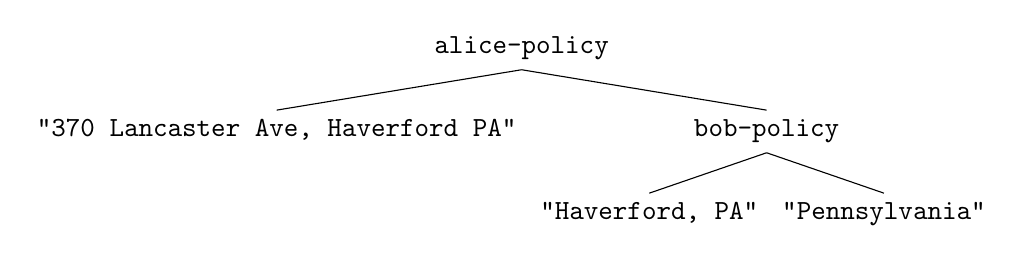
\begin{tikzpicture}
	\Tree
	[.\texttt{alice-policy}
		\texttt{"370 Lancaster Ave, Haverford PA"}
		[.\texttt{bob-policy}
			\texttt{"Haverford, PA"}
			\texttt{"Pennsylvania"}
		]
	]
	\end{tikzpicture}
\end{center}

Alice observes her nested facet in the usual way:

\begin{lstlisting}
(obs alice-policy "Alice" location-facet)
\end{lstlisting}

Bob must make two calls to \texttt{obs} to fully resolve the facet's value:

\begin{lstlisting}
(obs alice-policy "Bob" (obs bob-policy "Bob" location-facet))
\end{lstlisting}

As before, Bob must ensure that the policy he passes to each \texttt{obs} call matches the policy of the facet. In this case, the outer facet uses Alice's policy and the inner facet uses Bob's policy, so the calls to \texttt{obs} must be organized likewise.


\subsubsection{An example of faceted structs}
Compound data structures such as Racket structs may be faceted, however their behavior is somewhat counterintuitive. Take the following example:

\begin{lstlisting}
(struct emplyoyee (name position salary))
(define bob
  (employee "Bob" "manager" (fac bob-policy 70000 0)))
\end{lstlisting}

The call to the \texttt{employee} constructor is handled by \textsc{Racets} the way that any function call is: by branching execution on both values on the facet. Therefore, the return value is \texttt{(fac bob-policy (employee "Bob" "manager" 70000) (employee "Bob" "manager" 0))}, i.e. a facet that wraps two different instantiations of the \texttt{employee} struct. Bob's faceted salary can be accessed like so:

\begin{lstlisting}
(employee-salary (obs bob-policy "Bob" bob))
; or, equivalently:
(obs bob-policy "Bob" (employee-salary bob))
\end{lstlisting}

Somewhat surprisingly, \texttt{obs} is required to observe the name field (and any other field) of the \texttt{employee} object, even though it was not explicitly faceted in the constructor.

\begin{lstlisting}
(employee-name (obs bob-policy "Bob" bob))
\end{lstlisting}

\textsc{Racets} programs must take care to address these subtleties when working with faceted structs.


\subsubsection{An example of faceted lists}
Using faceted values with lists involves additional complications. Consider the following example:

\begin{lstlisting}
(define grades (list))
(set! grades (cons (fac alice-policy 84 0) grades))
\end{lstlisting}

As in the example with structs, the programmer likely intended for \texttt{grades} to be of the form \texttt{(list (fac alice-policy 84 0))}, i.e. a regular list containing a single facet. However, the real value of \texttt{grades} after the \texttt{set!} operation is

\begin{lstlisting}
(fac alice-policy (list 84) (list 0))
\end{lstlisting}

Imagine another grade was added to the list, like so:

\begin{lstlisting}
(set! grades (cons (fac bob-policy 73 0) grades))
\end{lstlisting}

Then the value of the list would be

\begin{lstlisting}
(fac bob-policy
  (fac alice-policy (list 73 84) (list 73 0))
  (fac alice-policy (list 0 84) (list 0 0)))
\end{lstlisting}

encompassing four different possibilities: satisfying both Alice and Bob's policies, satisfying one or the other, or satisfying neither.

The following procedure observes the entire list of grades into a regular Racket list of integers:

\begin{lstlisting}
(define (reveal-grades-rec grade-list policy-list arg)
  (if (empty? policy-list)
    grade-list
    (obs
      (car policy-list)
      arg
      (reveal-grades-rec
        grade-list
        (cdr policy-list)
        arg))))])
\end{lstlisting}

It takes in a list of grades, a list of policies which should correspond index-by-index to the list of grades (remember that \texttt{obs} requires the policy to match the facet's policy), and an argument to pass to the policy predicates.

This section and the previous one have illustrated fundamental issues with the interaction of faceted execution and data structures, stemming from the generic treatment of faceted function application. For the sake of programming ergonomics, future implementations of faceted execution may wish to not treat functional application quite so generically, to allow structure-creating forms like \texttt{list} and struct constructors to be special cases that behave more intuitively with faceted arguments.


\subsection{Syntactic macros}
The implementation of faceted execution in \textsc{Racets} relies heavily on a language feature called syntactic macros. Syntactic macros are a mechanism by which the source syntax of a program is transformed prior to execution. They are a more powerful cousin of the lexical macros familiar to C and C++ programmers. Racket, like most dialects of Lisp, includes a particularly powerful syntactic macro system. This section will briefly introduce the Racket macro system. Readers are referred to the ``Fear of Macros'' tutorial \cite{fear-of-macros} for a much more comprehensive overview.

A macro is defined like a function that takes a syntax object as input and outputs another syntax object, except the definition uses \texttt{define-syntax} instead of \texttt{define}. The simplest possible macro simply returns its input syntax unchanged:

\begin{lstlisting}
(define-syntax (identity stx)
  stx)
\end{lstlisting}

A macro is invoked just like a regular function:

\begin{lstlisting}
; Expands to just x
(identity x)
\end{lstlisting}

New syntax objects can be constructed with the \texttt{syntax} function or its abbreviation, \texttt{\#'}:

\begin{lstlisting}
(define-syntax (ignore-input stx)
  ; Equivalent to (syntax (displayln "ignoring input"))
  #'(displayln "ignoring input")
\end{lstlisting}

Syntax objects can be converted to and from lists. This functionality allows us to implement a macro that reverses its arguments:

\begin{lstlisting}
(define-syntax (reverse-syntax stx)
  (datum->syntax stx (reverse (cdr (syntax->datum stx)))))
\end{lstlisting}

A programmer could use the \texttt{reverse-syntax} macro as follows:

\begin{lstlisting}
; Expands to (+ 20 22), which evaluates to 42
(reverse-syntax 20 22 +)
\end{lstlisting}

\texttt{reverse-syntax} is the first example of a macro that could not be written as a regular Racket function, since it actually effects a transformation of the source syntax. Another example, familiar to users of the C preprocessor, accesses the location information that syntax objects carry to dynamically print the location of the macro invocation in the source code.\footnote{A similar effect can be achieved using the C preprocessor with the \texttt{\_\_LINE\_\_} and \texttt{\_\_FILE\_\_} macros.}

\begin{lstlisting}
(define-syntax (print-source-location stx)
  (datum->syntax
    stx
    `(displayln
       (format
         "line ~a of ~a"
         ,(syntax-line stx)
         ,(syntax-source stx)))))
\end{lstlisting}

More complicated macros can be written with the pattern-matching facilities of \texttt{syntax-case}. The following macro uses \texttt{syntax-case} to behave differently if it invoked with one argument or two:

\begin{lstlisting}
(define-syntax (one-or-two stx)
  (syntax-case stx ()
    [(_ a b)
     #'(displayln "Got two")]
    [(_ a)
     #'(displayln "Got one")]))
\end{lstlisting}

In the snippet above, each identifier in the \texttt{syntax-case} clause matches a single top-level expression (which may be an atomic value or a compound structure like a list). The underscore matches the name of the macro itself, and the symbols \texttt{a} and \texttt{b} match arguments to the macro.

One final point about syntactic macros in Racket is that they are hygienic, meaning that identifiers introduced in the macro are protected from conflicting with identifiers in the original source code. Consider the following macro in Racket:

\begin{lstlisting}
(define-syntax (hygienic stx)
  (syntax-case stx ()
    [(_ a)
     #'(let ([x 10]) (+ x a))]))
\end{lstlisting}

If \texttt{hygienic} was used in a context where another identifier \texttt{x} was defined, e.g.

\begin{lstlisting}
(define x 32)
(hygienic x)
\end{lstlisting}

then one might expect that it would expand to

\begin{lstlisting}
; Wrong!
(define x 32)
(let ([x 10] (+ x x)))
\end{lstlisting}

which would (counterintuitively) evaluate to 20. In actual fact, the macro system rewrites the identifier \texttt{x} in the macro to a name which it can guarantee will not collide with any existing identifier in the program, as demonstrated below.

\begin{lstlisting}
; Correct -- x in the macro is rewritten as x:3
(define x 32)
(let ([x:3]) (+ x x:3))
\end{lstlisting}

At runtime the expanded macro thus correctly evaluates to 42.

By contrast, macros in C are not hygienic, so in \texttt{swap} below, the \texttt{tmp} variable defined in the macro will interfere with unrelated uses of \texttt{tmp} in the same scope as the macro invocation.

\begin{lstlisting}[language=C]
#define swap(x, y) int tmp = x; x = y; y = tmp;
\end{lstlisting}

Hygienic syntactic macros are a powerful feature of the Racket language that will be leveraged in section \ref{sec:lang} to implement faceted execution in a seamless manner that would not be possible in a language that did not expose a rich set of mechanisms for language extension.



\section{Type theory}
Programmers must be careful to apply the correct policies when they observe faceted values. Since the \textsc{Racets} language is dynamically typed, errors in the use of faceted execution are not caught until runtime. A static type system for faceted values would be able to more reliably catch programmer errors.

The definition of a type system is ``a tractable syntactic method for proving the absence of certain program behaviors by classifying phrases according to the kinds of values they compute'' \cite{types}. The program behaviors that a type system are meant to prevent are generally what are called type errors: attempted operations on values for which the operation is not defined.

Naturally, some undesirable program behaviors cannot be detected by a static type system (e.g., looping infinitely is not detectable due to the uncomputability of the halting problem), and type systems will sometimes refuse to accept constructs which are in fact safe. Nonetheless, a well-designed type system is an effective tool for catching programmer errors.

A simple model of a static type system is the typed lambda-calculus. The following exposition is based on chapter 9 of \cite{types}.

The lambda calculus is a simple model of calculation in which the only data type is the function and the only operation is function application. Syntactically the lambda calculus has three kinds of terms: variables ($x$, $y$, etc.), anonymous functions, also known as abstractions ($\lambda x . x$), and function applications ($t\ t$). The notation $\lambda x . x$ is equivalent to the more traditional notation of $f(x) = x$, except that it has the advantage of not requiring the function to be named. Function application of the form $t_1\ t_2$ is equivalent notationally to $t_1(t_2)$. The body of a lambda function may contain any of the three syntactic forms of the language, so for example $\lambda x . \lambda y . (\lambda z . z)(x)$ is a valid term in the lambda calculus whose outermost abstraction contains another abstraction, which in turn contains an application. For clarity, the application is written with parentheses.

The typed lambda calculus has the same syntax as the untyped lambda calculus, except that a type annotation is necessary for lambda abstractions, which are now written as $\lambda x: T . x$ instead of $\lambda x. x$, where $T$ is a type. The $: T$ syntax is an example of a \textit{type annotation}---an annotation supplied by the programmer that indicates the intended type of a variable or expression. Not all languages require type annotations, but they are often beneficial for clarity and simplicity of implementation.

A type system for the lambda calculus (and indeed for any programming language) must assign a type to each syntactic construction in the language. These assignments are formally known as type rules. Type rules are written in the form

\[
\frac{\text{hypotheses}}
{\text{conclusion}}
\]

where \textit{hypotheses} is a set of assumptions and \textit{conclusion} is a type judgment that follows from the hypotheses.

The rule for the types of variables is\footnote{The type rules are taken from Figure 9-1 on p. 103 of \cite{types}.}

\[
\frac{x : T \in \Gamma}
{\Gamma \vdash x : T}
\]

$\Gamma$ stands for an assignment function that maps from a finite number of variable names to their values. The notation $\Gamma \vdash t : T$ expresses the three-place typing relation that syntactic term $t$ has type $T$ given the assignment $\Gamma$. The type rule for variables simply states that if a variable is paired with a certain type $T$ in the assignment function, then $T$ is the variable's type.

The rule for lambda abstraction is a bit more complicated:

\[
\frac{\Gamma, x : T_1 \vdash t_2 : T_2}
{\Gamma \vdash \lambda x : T_1 . t_2 : T_1 \to T_2}
\]

In the hypothesis $\Gamma, x : T_1$ should be read as ``$\Gamma$ augmented with the assignment of type $T_1$ to $x$.'' It is assumed that the variable $x$ is not already in $\Gamma$; if it is, it can simply be renamed. The full hypothesis of the abstraction rule thus states that the body of the lambda function has type $T_2$ with the given assignment function. The conclusion of the abstraction rule states that the lambda function as a whole has the complex type $T_1 \to T_2$.

Finally, the last syntactic form of the language, application, has the type rule

\[
\frac{\Gamma \vdash t_1 : T_{11} \to T_{12}\ \ \ \ \ \ \Gamma \vdash t_2 : T_{11}}
{\Gamma \vdash t_1\ t_2 : T_{12}}
\]

Given that the function has type $T_{11} \to T_{12}$ in $\Gamma$, and the argument has type $T_{11}$, then the expression as a whole has type $T_{12}$.

The three type rules presented above can be applied to any expression in the typed lambda calculus to detect whether it is well-typed, and if it is, to determine its concrete type. Thus the type system is able to statically eliminate a class of errors from the simple lambda calculus.

Type systems for real programming languages are significantly more complex, but involve the same basic formalism of inference rules and type judgments.



\section{Extending Racket with faceted execution\label{sec:lang}}
Racket provides several ways to extend its syntax and semantics. The current implementation of \textsc{Racets} uses syntactic macros. A more flexible and powerful approach using Racket's \texttt{\#lang} will also be presented.


\subsection{Racets with macros}
At present, the \textsc{Racets} system is implemented as a set of syntactic macros in Racket. The macros redefine core Racket constructs like \texttt{lambda}, \texttt{if}, and \texttt{\#\%app} (function application) to make them sensitive to faceted values. For example, the \texttt{lambda} form is transformed by the \texttt{fac-lambda} macro, which wraps the resulting function in a special data structure.

\begin{lstlisting}
(define-syntax (fac-lambda stx)
  (syntax-parse stx
    [(_ xs expr)
      #'(fclo (lambda xs expr))]))
\end{lstlisting}

Other macros are provided for a subset of the core forms of Racket. See \cite{racets} for details of the implementation.


\subsubsection{Shortcomings}
Implementing \textsc{Racets} using macros suffers from two shortcomings: it is not possible to transform bare identifiers, and the \textsc{Racets} macros may interfere with user-defined or third-party macros.

To correctly handle faceted execution, the \textsc{Racets} system needs to wrap (some) identifiers with the \texttt{facet-deref} form. To see why, consider the following code block:

\begin{lstlisting}
(if k
  (set! x 100)
  (set! x 0))
\end{lstlisting}

Suppose that \texttt{k} is a facet belonging to Alice whose high-confidentiality value is true and whose low-confidentiality value is false. Upon execution of the \texttt{if} statement, the value of \texttt{x} will be a box that contains the facet $\langle \textit{alice}\ ?\ 100 : 0 \rangle$. However, subsequent references to \texttt{x} will assume that it is of integer type, and without a \texttt{facet-deref} transformation to extract the underlying facet from the box, these references may cause the code fail.

Note that this is a different problem from invisibly transforming regular values into facets, as was done in many of the examples of section \ref{sec:facets}. Faceted values are automatically handled by the faceted execution mechanism, e.g. the re-defining of the \texttt{\#\%app} macro to work for facets. The problem here is that the use of the \texttt{set!} form (which expands to \texttt{facet-set!} in \textsc{Racets}) results in \texttt{x} becoming a box containing a facet and not just a bare facet.

It is simply not possible to target bare identifiers with a syntactic macro because identifiers are ``raw'' in the syntax: unlike function applications, lambda definitions, and other Racket constructs, identifiers are not wrapped in an identifier-specific syntactic form at any point in the expansion process, and thus it is impossible for a macro to target them specifically and exclusively, at least in the way that, e.g., \texttt{\#\%app} can target every function application.


\subsection{Racets as a language-as-a-library}
These shortcomings can be averted with \textsc{Racets}'s \texttt{\#lang} mechanism. Source files in Racket typically begin with a \texttt{\#lang racket} declaration. However, other languages may be defined (e.g., \texttt{\#lang typed/racket} \cite{typed-racket}) which reuse some of the syntax and semantics of Racket and modify other parts of it, down to the level of lexical structure.

The language-as-a-library approach \cite{typed-racket} uses \texttt{\#lang} to implement new domain-specific languages which are typically compatible with Racket code and which are much easier to write than a new language from scratch, since they can make use of all the facilities exposed by the Racket compiler.

The key idea of languages-as-libraries is to override the \texttt{\#\%module-begin} form (which wraps all Racket modules), and use a Racket function called \texttt{local-expand} to simplify the module's contents into a minimal subset of Racket called Fully-Expanded Racket \cite{fe-racket}. The language designer then need only provide translations for the small set of core forms that constituted Fully-Expanded Racket.


\subsubsection{Small example of a language-as-a-library}
The following minimal but complete example of the languages-as-libraries idea prints out the fully-expanded abstract syntax tree of a program before running it normally:

\begin{lstlisting}
#lang racket

; Fully expands the module and prints out its abstract syntax
; tree, before running it normally.
(define-syntax (module-begin stx)
  (syntax-case stx ()
    [(_ forms ...)
    (with-syntax ([(_ core-forms ...)
                   (local-expand
                     #'(#%plain-module-begin forms ...)
                     'module-begin
                     '())])
      #'(#%plain-module-begin
          (displayln '(core-forms ...))
          core-forms ...))]))

; Export everything from the regular Racket language, except
; replaced #%module-begin with our own implementation.
(provide (except-out (all-from-out racket) #%module-begin)
  (rename-out [module-begin #%module-begin]))
\end{lstlisting}

If this program were saved in a file called \texttt{racket/print-ast.rkt}, then other files could be written in the language by beginning with \texttt{\#lang s-exp "racket/print-ast.rkt"} instead of \texttt{\#lang racket}.

The language file begins with the standard \texttt{\#lang racket} declaration, since the file itself is written in Racket. It then defines a macro called \texttt{module-begin} which rewrites its syntax object to be

\begin{lstlisting}
#'(#%plain-module-begin
    (displayln '(core-forms ...))
    core-forms ...))]))
\end{lstlisting}

where \texttt{core-forms} is defined by the \texttt{with-syntax} clause to be the result of invoking \texttt{local-expand} on the original syntax object. The macro then outputs a \texttt{\#\%plain-module-begin} form (rather than a \texttt{\#\%module-begin}, to avoid infinite recursion) that wraps the original source syntax, after a call to \texttt{displayln} that prints at run-time the actual syntax object that was generated at compile-time.


\subsubsection{Larger example of a language-as-a-library}
As a proof-of-concept of implementing Racets with the language-as-a-library approach, this section presents a library called \texttt{wrap-ident.rkt} that rewrites identifiers in the source code so that the text of the identifier is printed out whenever it is evaluated. For example, running the module below would generate the output \texttt{Dereferencing x  Dereferencing y}.

\begin{lstlisting}
#lang s-exp "wrap-ident.rkt"

(define x 10)
(define y 32)
(displayln (+ x y))
\end{lstlisting}

The \texttt{wrap-ident.rkt} defines two helper functions, \texttt{transform-syntax} and \texttt{wrap-variable}, which together transform the AST in the prescribed manner. Since these functions are used by a macro (but are not themselves macros), they must be wrapped in a \texttt{begin-for-syntax} block:

\begin{lstlisting}
#lang racket

(require (for-syntax racket/match))

(begin-for-syntax
  (define (wrap-variable v)
    (let ([vstr (symbol->string v)])
      (quasiquote
        (begin
          (display "Dereferencing ") (displayln ,vstr) ,v))))

  (define (transform-syntax datum)
    (match datum
      [(list '#%app f xs ...)
        (cons
          f
          (map
            (lambda (x)
              (if (symbol? x)
                (wrap-variable x)
                (transform-syntax x)))
            xs))]
      [(list xs ...) (map transform-syntax xs)]
      [default default])))
\end{lstlisting}

\texttt{(wrap-variable p)} evaluates to \texttt{(begin (display "Dereferencing) (displayln "p") p)}. \texttt{transform-syntax} recursively traverses the AST and rewrites symbols using \texttt{wrap-variable}. In the implementation above, only function applications (represented by the \texttt{\#\%app} base form in fully-expanded Racket) have their identifiers re-written. A full implementation of this language would have a separate case for each of the base forms in fully-expanded Racket that could potentially take an identifier argument.

The final piece is the whole-module rewrite rule:

\begin{lstlisting}
(define-syntax (module-begin stx)
  (syntax-case stx ()
    [(_ forms ...)
      (let ([as-datum
              (syntax->datum
                (local-expand
                  #'(#%plain-module-begin forms ...)
                  'module-begin
                  '()))])
        (datum->syntax stx (transform-syntax as-datum)))]))

(provide (except-out (all-from-out racket) #%module-begin)
         (rename-out [module-begin #%module-begin]))
\end{lstlisting}

The \texttt{module-begin} macro invokes \texttt{local-expand} on the module contents, and then converts the syntax object into a list using \texttt{syntax->datum}. The \texttt{transform-syntax} function is invoked on the list, and the result is converted back to a syntax object.



\section{Abstract interpretation}
A practical problem of implementing faceted execution is that it can have high runtime cost. As the example with \texttt{square-root} in section \ref{sec:facets} indicated, functions applied to facets must be evaluated twice, once with the high-confidentiality value and once with the low-confidentiality value. The double evaluation imposes a significant runtime cost on faceted execution (as well as complicating the use of functions with side-effects). This cost can be mitigated to some extent by static analysis. If the static analyzer can prove that a facet passed to a function only ever evaluates to its high-confidentiality value, then the evaluation of the function with the low-confidentiality value could be skipped, and significant performance gains could be realized.

One technique for static analysis is abstract interpretation, wherein the computation of a program is modelled with abstract objects (e.g., the abstract ``negative number'' instead of the concrete $-10$) so that real properties of the program can be reasoned about \cite{ai-original}. Abstract interpreters can be derived mechanically from abstract machines, provided that the formalism for the abstract machine is expressed in an amenable manner \cite{aam}. An abstract interpreter of a \textsc{Racets}-like language is under development for this purpose \cite{abstract-inter}.

The level of detail that the abstract interpreter attains with its analysis can have a substantial effect on performance. For example, if a certain function is sometimes applied to faceted values and sometimes applied to regular values, the abstract interpreter may or may not be able to identify the call sites that require special handling of the faceted execution, and those that can be run normally. In general, the more fine-grained the conclusions the abstract interpreter can draw, the greater the improvement of performance time, at the cost of slower analysis and a more complex abstract interpreter.

TODO: More details about the abstracting abstract machines approach.
TODO: Show how a small example program is transformed by the Racets macros, and point out how abstract interpretation could simplify it.



\section{Conclusion}
This thesis has identified three areas in which the ergonomics of faceted execution could be improved: faceted code is slower than non-faceted code, it is easy to make avoidable mistakes when using the \texttt{obs} form, and present implementations of faceted execution have trouble integrating smoothly with external (i.e., non-faceted) code. I have reviewed potential solutions for each of these problems: static analysis by abstract interpretation to reduce runtime overhead, static typing to catch programmer errors, and Racket's \texttt{\#lang} mechanism to ease compatibility with non-faceted code. Additionally, I have shown how the present implementation of \textsc{Racets} could be re-written using \texttt{\#lang}. The techniques and theory reviewed in this thesis should contribute to making writing code with faceted execution more ergonomic, and thus indirectly to safeguarding the privacy of software users.

% TODO: Bib entry for FE Racket looks terrible
\bibliography{thesis}

\end{document}
